\section{Introduction}

%===========================================================================================
% Motivation
%===========================================================================================
Now that intelligence with reinforcement learning has been shown to be superior to humans \citep{tesauro1995temporal,mnih2015human,silver2016mastering}, reinforcement learning is expected to expand into industry applications such as stock trading, autonomous cars, smart grids, and IoT. 
In future industrial applications, numerous companies will own agents used to improve their revenues.
Such a situation can be considered as each agent independently solving the problems of a partially observed Markov decision process (POMDP).

These company agents are designed to independently maximize their own rewards; 
however, if such agents could exchange information, the overall revenue of stakeholders would increase.
As each agent has limited visibility of the environment, information exchanges between agents would be helpful in solving their independent tasks.
Thus, this paper aimed to actualize a society where stakeholders with conflicting interests willingly trade information.

We regard the situation as communication in multi-agent reinforcement learning (MARL).
Multi-agent communication is addressed by several methods such as R/DIAL \citep{foerster2016learning} and CommNet \citep{sukhbaatar2016learning}.
CommNet is a state-of-the-art MARL method that considers communication between agents 
and features learning among agents with backpropagation.

When considering conditions in MARL such that different stakeholders have created different agents that communicate with each other, an reward distribution design (e.g., monetary payment) and a framework without a {\em trusted third party} (TTP) are required.
TTP \citep{wu1999game,sandholm2002possibility} is a neutral administrator that performs reward distributions for all participants, and is supposed implicitly by most existing literature regarding MARL \citep{agogino2006quicr,foerster2016learning,sukhbaatar2016learning}.
Although there is a requirement for TTP neutrality towards all participants,
several peer-to-peer trade configurations, such as inter-industry and -country trades, cannot place TTP.
If reward distribution is performed by an untrusted third party, the rewards for partial participants may be undesirably altered.

To the best of our knowledge, no existing literature discusses reward distributions in the configuration described above.
Because CommNet assumes an environment that distributes a uniform reward to all the agents, 
if the distributed reward is in limited supply (such as money), it causes the {\em Tragedy of the Commons} \citep{lloyd1833two}, where the reward of contributing agents will be reduced due to the participation of free riders.
Although there are several MARL methods for distributing rewards according to agents' contribution such as QUICR \citep{agogino2006quicr} and COMA \citep{sukhbaatar2016learning}, they suppose the existence of TTP and hence cannot be applied to the situation investigated here.

%===========================================================================================
% Objective
%===========================================================================================

The proposed method, {\em Neuron as an Agent} (NaaA), extends CommNet to actualize reward distributions
in MARL without TTP based on two key ideas: (i) inter-agent reward distribution and (ii) auction theory.
Auction theory was introduced because inter-agent reward distributions were insufficient for optimization.
Agents in NaaA maximize {\em profit}, the difference between their received rewards and the costs which they redistribute to other agents.
If the framework is naively optimized, a trivial solution is obtained where agents reduce their costs to zero to maximize profits.
Then, NaaA employs the auction theory in game design to prevent costs from dropping below their necessary level.
As a theoretical result, we show that agents autonomously evaluate the {\em counterfactual return} as values of other agents.
The counterfactual return is equal to the discounted cumulative sum of counterfactual reward \citep{agogino2006quicr} distributed by QUICR and COMA.
%NaaA actualizes reward distributions, making it more of a pareto improvement than inter-agent reward distribution method.

\begin{figure*}[tb]
	\centering
	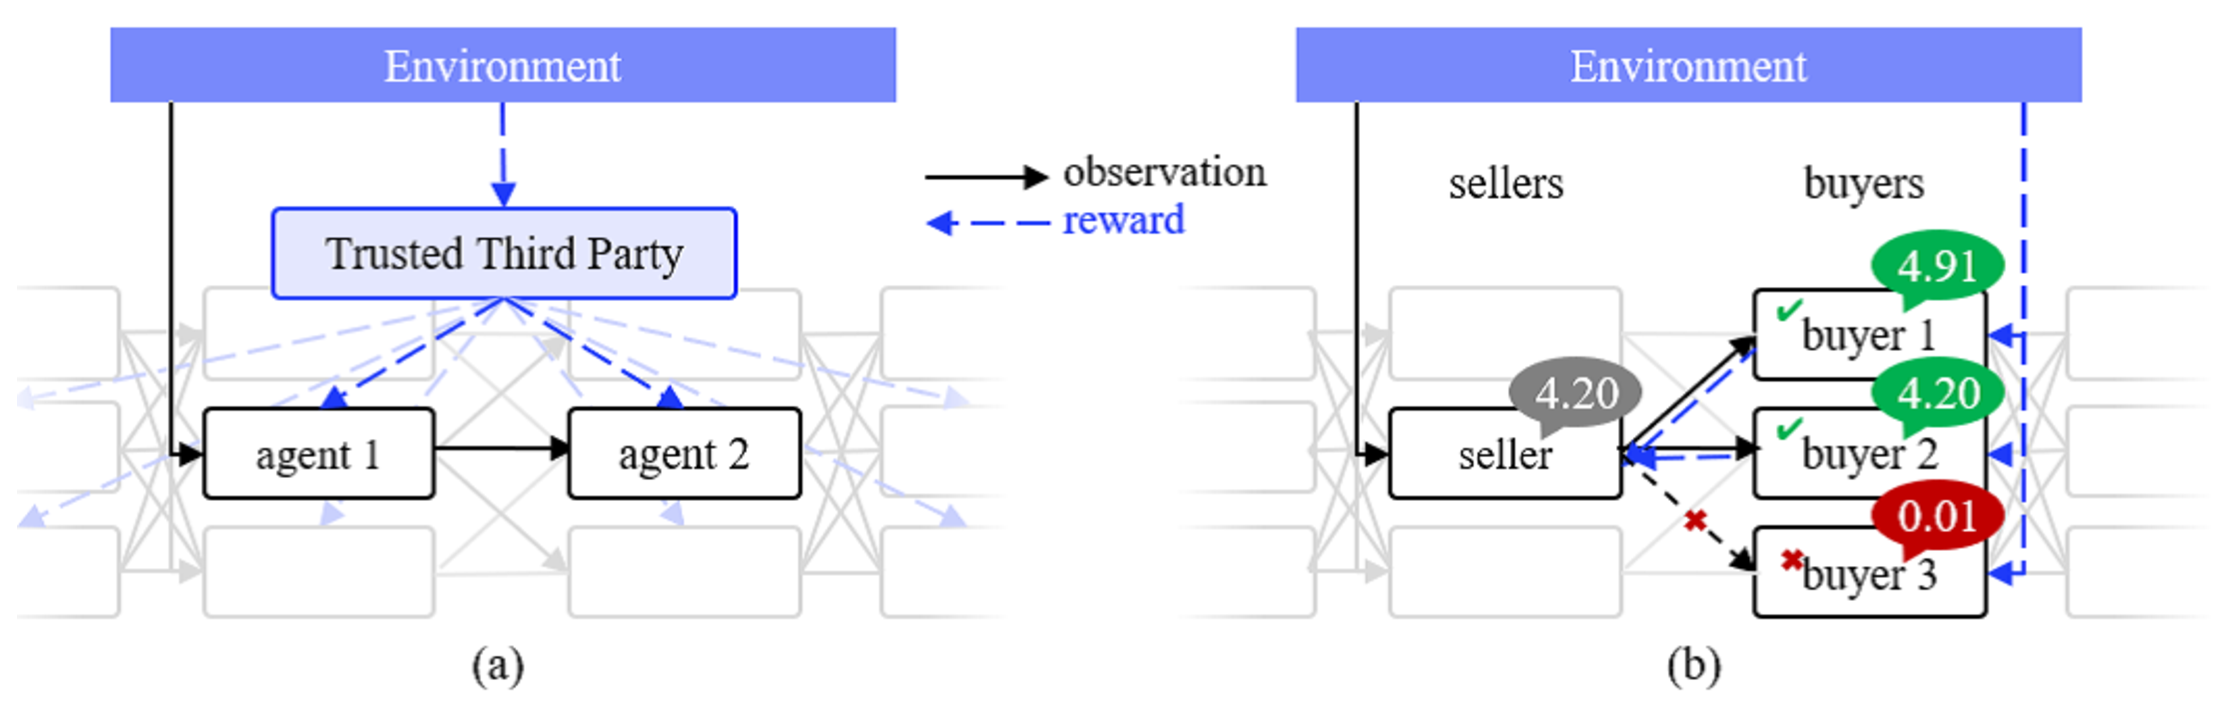
\includegraphics[width=\linewidth]{img/TTP.eps}
	\caption{
		A schematic illustration of reward distribution models in MARL.
		{\bf (a)} Centralized reward distribution model \citep{agogino2006quicr,sukhbaatar2016learning,foerster2016learning,foerster2017counterfactual}. They should suppose TTP to distribute the optimal reward to the agents. % receives reward from the environment directly, and distribute the agent  The optimal reward is calculated by the TTP.
		{\bf (b)} Inter-agent reward distribution model (our model). Some agents receive reward from the environment directly, and redistribute to other agents. The idea to determine the optimal reward without TTP is playing auction game among the agents.
			%The agents maximize their profit instead of reward.
		%{\bf (c)} Neuron as an Agent (NaaA). Inter-agent reward distribution includes reward backpropagation along the connections. 
	}
	\label{fig:ttp}
\end{figure*}

NaaA enables representation trades in peer-to-peer environments and, ultimately, regards neural network units as agents.
As NaaA is capable of regarding units as agents without losing generality, this setting was utilized in the current study.
The concept of the proposed method is illustrated in \figurename~\ref{fig:ttp}.

An environment extending ViZDoom \citep{kempka2016vizdoom}, a POMDP environment, to MARL was used for the experiment.
Two agents, a cameraman sending information and a main player defeating enemies with a gun, were placed in the environment.
Results confirmed that the cameraman learned cooperative actions for sending information from dead angles (behind the main player) and outperformed CommNet in score.

Interestingly, NaaA can apply to single- and multi-agent settings, since it learns optimal topology between the units. %with respect to supervised learning
{\em Adaptive DropConnect} (ADC), which combines DropConnect \citep{wan2013regularization} (randomly masking topology) with an adaptive algorithm (which has a higher probability of pruning connections with lower counterfactual returns) was proposed as a further application for NaaA.
Experimental classification and reinforcement learning task results showed ADC outperformed DropConnect.
%Subsequently, we present that our trading model leads the model to learning optimal topology between the units with respect to supervised learning as well as MARL.
%It uses $\varepsilon$-greedy as an exploration policy, and is equivalent to DropConnect in the case of $\varepsilon = 1$. It is equivalent to counterfactual return maximization, which constructs the topology deterministically in the case of $\varepsilon = 0$.

% Organization
The remainder of this paper is organized as follows. 
In the next section, we show the problem setting.
Then, we show proposed method with two key ideas: inter-agent reward distribution and auction theory in Section 3. 
After related works are introduced in Section 4, the experimental results are shown in classification, single-agent RL and MARL in Section 5.
Finally, a conclusion ends the paper.
